\documentclass[14pt]{extarticle}

\usepackage[T2A]{fontenc}
\usepackage[utf8]{inputenc}
\usepackage[russian]{babel}
\usepackage{graphicx}
\usepackage{caption}
\DeclareCaptionLabelSeparator{dot}{. }
\captionsetup{justification=centering,labelsep=dot}
\usepackage{amsmath}
\usepackage{amssymb}
\input glyphtounicode.tex
\input glyphtounicode-cmr.tex
\pdfgentounicode=1
\usepackage{bm}

\begin{document}

ФИО: Медяков Даниил Олегович

\vspace{10pt}

Номер задачи: 53

\vspace{10pt}

Решение:

\vspace{10pt}
Для начала запишем функцию правдоподобия для обеих гипотез:
\begin{equation*}
    L_1(x) = f_{\mathcal{N}(-1,1)}(x) = \frac{1}{\sqrt{2\pi}}\exp\left(-\frac{(x + 1)^2}{2}\right)
\end{equation*}
\begin{equation*}
    L_2(x) = f_{\mathcal{N}(2,4)}(x) = \frac{1}{\sqrt{8\pi}}\exp\left(-\frac{(x - 2)^2}{8}\right)
\end{equation*}

Теперь мы можем составить функцию отношения правдоподобия:

\begin{eqnarray*}
    \begin{split}
        l(x)=\frac{L_2(x)}{L_1(x)}=\frac{\exp\left(-\frac{(x - 2)^2}{8}\right)}{2\cdot \exp\left(-\frac{(x + 1)^2}{2}\right)}= \frac{1}{2} \cdot \exp \left(-\frac{(x-2)^2}{8}+\frac{(x+1)^2}{2}\right) =
        \\=
        \frac{1}{2} \cdot \exp \left(\frac{1}{8} \cdot\left(3 x^2+12 x\right)\right)= \frac{1}{2} \cdot \exp \left(\frac{3}{8} \cdot\left(\left(x+2\right)^2-4\right)\right)=
        \\ = \frac{1}{2}\cdot \exp \left(\frac{3}{8}(x+2)^2\right) \cdot e^{-3 / 2}        
    \end{split}
\end{eqnarray*}

Из леммы Неймана-Пирсона следует, что наиболее мощный критерий с уровнем значимости $\alpha \leq \mathbb{P}_1(l(x) > c) \equiv 1$ можно искать среди критериев вида
\begin{eqnarray*}    
    \pi_{c, p}(x)=
    \begin{cases}
    1, l(x)>c \\
    p, l(x)=c \\
    0, l(x)<c.
\end{cases}
\end{eqnarray*}

Из условия на уровень значимости, а именно 
\begin{equation*}
    \mathbb{P}_1(l(x)>c)+p \cdot \mathbb{P}_1(l(x)=c)=\alpha,
\end{equation*}

найдем конкретные значения $c > 0 $ и $p \in [0,1]$.

Поскольку распределение $N(-1,1)$ абсолютно непрерывно, то \\ $\mathbb{P}_1(l(x)=c)=0$. $p$ можно выбрать любым, например, $p=0$. Условие на  $c$ определим из уравнения: $\mathbb{P}_1[l(x)>c]=\alpha$.

\begin{gather*}
        l(x)>c  \Leftrightarrow  \frac{\exp \left(\frac{3}{8}(x+2)^2\right)}{2}e^{-3 / 2}  >c \Leftrightarrow 
        \\ \Leftrightarrow
        (x+2)^2>\frac{8}{3} \ln \left(\frac{2c}{e^{-3 / 2}} \right)=R^2>0
        \\
        x \in N(-1,1) \Rightarrow 
        \\        \mathbb{P}_1(l(x)>c)=\mathbb{P}_1\left((x+2)^2>R^2\right)=\mathbb{P}_1(x>R-2)+\mathbb{P}_1(x<-2-R)=\alpha
\end{gather*}


Подставим выражения функций рапсределения для вычисления значения $R$:

\begin{gather*}
\left(1-\mathcal{F}_{\mathcal{N}(-1, 1)}(R-2)\right)+\mathcal{F}_{\mathcal{N}(-1, 1)}(-2-R)=\alpha, 
\\
\mathcal{F}_{\mathcal{N}(-1, 1)}(R-2)-\mathcal{F}_{\mathcal{N}(-1, 1)}(-2-R)=1-\alpha.
\end{gather*}

В условии задачи также просят построить зависимость ошибки второго рода от $\alpha$, подсчитаем чему будет равна $\beta$ :
\begin{gather*}
\mathbb{E}_2\left[\pi\right]=1 \cdot \mathbb{P}_2\left((x+2)^2>R^2\right)=\mathbb{P}_2(x>R-2)+\mathbb{P}_2(x<-2-R) \\
1-\mathbb{E}_2\left[\pi\right]=1-\mathbb{P}_2(x>R-2)-\mathbb{P}_2(x<-2-R)= \beta \\
\Rightarrow  \mathcal{F}_{N(2,4)}(R(\alpha)-2)-\mathcal{F}_{N(2,4)}(-2-R(\alpha))= \beta
\end{gather*}
Ответ:

\quad\quad\quad\quad\quad\quad\quad\quad$R=2.2845$,
\begin{eqnarray*}
    \pi(x)
    \begin{cases}
    1, \text{ при } x^2>R^2 \\
    0, \text{ при } x^2 \leqslant R^2.
    \end{cases}
\end{eqnarray*}

Также построим график зависимости $\beta(\alpha)$:
\begin{figure}
\begin{center}
	{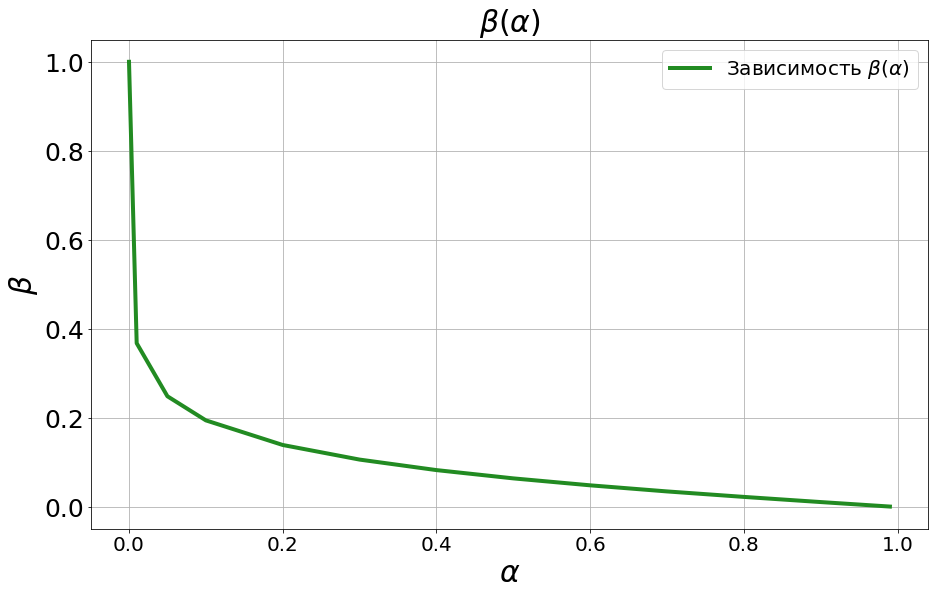
\includegraphics[scale=0.5]{Medyakov53.png}}
\end{center}
\end{figure}
\end{document}